\documentclass{article}
\usepackage[utf8]{inputenc}
\usepackage[T2A]{fontenc}
\usepackage[russian]{babel}
\usepackage[normalem]{ulem}
\usepackage{amsfonts}
\usepackage{amsmath}
\usepackage{amsthm}
\usepackage{amssymb}
\usepackage{arcs}
\usepackage{fancyhdr}
\usepackage{float}
\usepackage[left=2cm,right=2cm,top=2cm,bottom=2cm]{geometry}
\usepackage{graphicx}
\usepackage{hyperref}
\usepackage{multicol}
\usepackage{stackrel}
\usepackage{xcolor}
\usepackage{cancel}

\makeatother
\makeatletter

\title{\textbf{Билеты к коллоку}}
\author{i.g. i.a.}
\date{20 марта 2023 г.}

\DeclareMathOperator*\lowlim{\underline{lim}}
\DeclareMathOperator*\uplim{\overline{lim}}

\newcommand*{\limToInf}[2]{\displaystyle \lim_{#1 \to \infty} #2}
\newcommand*{\limToZero}[2]{\displaystyle \lim_{#1 \to 0} #2}
\newcommand*{\lemma}[1]{\textbf{Лемма.} #1. \newline}
\newcommand*{\theorem}[2]{\textbf{Теорема #1. } #2 \newline}
\newcommand*{\notabene}[1]{\textit{Notabene. #1.} \newline}
\newcommand*{\definition}[1]{\textbf{Определение.} #1 \newline}
\newcommand*{\R}{\mathbb{R}}
\newcommand*{\eps}{\varepsilon}
\newcommand*{\cf}[2]{\cfrac{#1}{#2}}
\newcommand*{\D}{\Delta}
\newcommand*{\p}[1][n]{P_{#1}(x)}
\newcommand*{\Q}[1][m]{Q_{#1}(x)}
\newcommand*{\Rfrac}[2]{\frac{\p{#1}}{\Q{#2}}}
\newcommand*{\sfrac}{\frac{A}{(x - a)^k}}
\newcommand*{\Sfrac}{\frac{Ax+B}{(x^2 + px + q)^k}}
\newcommand*{\PAdv}[2]{P_{#1}^{#2}(x)}
\newcommand*{\QAdv}[2]{Q_{#1}^{#2}(x)}
\begin{document}
\tableofcontents
\maketitle

\section{Понятие первообразной. Теорема о двух первообразных. Понятие неопределенного интеграла.}

\textbf{Замечание: } Ниже под обозначением $\langle a, b \rangle$ будет пониматься произвольный промежуток: отрезок, интервал или полуинтервал.
\newline
\newline
\definition{Первообразной функции $f(x)$ на промежутке $\langle a, b \rangle$ называется функция $F(x)$ такая, что для всех $x \in \langle a, b \rangle$ выполняется равенство: }
$$
    F'(x) = f(x)
$$
\textbf{Несколько примеров: } 
\begin{enumerate}
    \item Пусть $f(x) = x^2$, тогда первообразная $F(x) = \cfrac{x^3}{3}$;
    \item Пусть $f(x) = \sin x$, тогда $F(x) = -\cos x$;
    \item Пусть $f(x) = 0$, тогда $F(x) = C$, $C \in \R$. 
\end{enumerate}
и так далее.
\newline 
\newline 
\theorem{(о двух первообразных)}{Пусть $F(x)$ - первообразная функция $f(x)$ на $\langle a, b \rangle$. Для того, чтобы $\Phi(x)$ также была первообразной для $f(x)$ на $\langle a, b \rangle$, необходимо и достаточно, чтобы}
$$
    F(x) - \Phi(x) \equiv C, \quad \forall x \in \langle a, b \rangle
$$
\begin{proof}
    Необходимость. Пусть $\Psi(x) = F(x) - \Phi(x)$, где $F(x), \Phi(x)$ - первообразные $f(x)$ на $\langle a, b \rangle$. Тогда $\forall x \in \langle a, b \rangle$:
    $$
        \Psi'(x) = (F(x) - \Phi(x))' = F'(x) - \Phi'(x) = f(x) - f(x) = 0
    $$
    По следствию из теоремы Лагранжа, для любых $x_1, x_2 \in \langle a,b \rangle$ таких, что $x_1 < x_2$
    $$
        \Psi(x_2) - \Psi(x_1) = \Psi'(\xi)(x_2 - x_1) = 0, \quad \xi \in (x_1, x_2) 
    $$
    тогда $\Psi(x) \equiv const$
    \newline
    \newline 
    Достаточность. Пусть $F(x) - \Phi(x) = C$ выполнено, тогда $\Phi(x) = F(x) + C$ и тогда
    $$
        \Phi'(x) = F'(x) + C' = F'(x) + 0 = f(x)
    $$
    значит $\Phi(x)$ - первообразная $f(x)$ на $\langle a, b \rangle$.
\end{proof}
.
\newline
\definition{Неопределенным интегралом функции $f(x)$ на промежутке $\langle a, b \rangle$ называется \textit{множество всех первообразных на этом промежутке}. Обозначается:}
$$
    \int f(x)dx
$$
Также это значит, что 
$$
\int f(x)dx = F(x) + C
$$
\definition{Функция $F(x)$ называется \textit{обобщенной первообразной} $f(x)$ на $\langle a, b \rangle$, если $F(x)$ - непрерывна на $\langle a, b \rangle$ и $F'(x) = f(x)$ везде, кроме не более чем конечного числа точек.}
\section{Таблица неопределенных интегралов.}
\begin{figure}[!ht]
    \begin{center}
    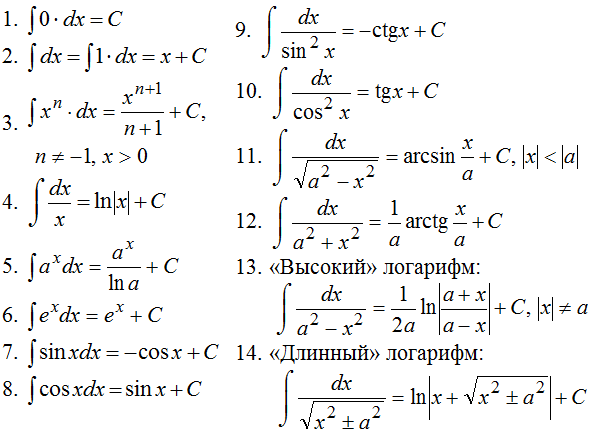
\includegraphics[scale=0.6]{unkn_inttbl.png}\caption{Таблица неопределенных интегралов.}\label{Таблица неопределенных интегралов.}
    \end{center}
\end{figure}
.\newline
Доказательство каждого из них состоит в том, что нужно продифференцировать правую часть\dots \textbf{!!ВЫУЧИТЕ ТАБЛИЦУ!!}
\section{Свойства неопределенного интеграла.}
ladies and gentlemans:
\begin{enumerate}
    \item \theorem{(связь с производной)}{Пусть $\int f(x)dx$ на $\langle a, b \rangle$, тогда на $\langle a, b \rangle$: }
    \begin{enumerate}
        \item $(\int f(x)dx)' = f(x)$;
        \item $d(\int f(x)dx) = f(x)dx$.
    \end{enumerate}
    \begin{proof}
        1, 2)
        $$
            \Bigl(\int f(x)dx \Bigr)' = (F(x) + C)' = f(x)
        $$
        Напомним, что $df = f'(x)dx$ и все становится очевидно.
    \end{proof}
    \item \lemma{Если $F(x)$ интегрируема на $\langle a, b \rangle$, то $\int dF(x) = F(x) + C$}
    \item \theorem{(линейность)}{Пусть на $\langle a, b \rangle$ существуют неопределенные интегралы $\int f(x)dx$ и $\int g(x)dx$, $\alpha^2 + \beta^2 \neq 0$. Тогда}
    $$
        \int (\alpha f(x) + \beta g(x))dx = \alpha\int f(x)dx + \beta\int f(x)dx
    $$
    \begin{proof}
        По предыдущему свойству,
        $$
            \Bigl(\alpha \int f(x)dx + \beta \int g(x)dx \Bigr)' = \alpha f(x) + \beta g(x)
        $$
        проинтегрировав обе части получим, что 
        $$  
            \alpha\int f(x)dx + \beta\int f(x)dx = \int (\alpha f(x) + \beta g(x))dx
        $$
    \end{proof}
    \item \theorem{формулы замены переменной}{Пусть на $\langle a, b \rangle$ существует неопределенный интеграл $\int f(x)dx, \; \varphi(t) \; : \; \langle \alpha, \beta \rangle \to \langle a, b \rangle$, дифференцируема на $\langle \alpha, \beta \rangle$, тогда}
    $$
        \int f(x)dx = \int f(\varphi(t))\varphi'(t)dt 
    $$
    \begin{proof}
        Пусть $F(x)$ - первообразная для функции $f(x)$ на $\langle a, b \rangle$, тогда, согласно теореме о производной сложной функции, $F(\varphi(t))$ - первообразная для функции $f(\varphi(t))\varphi'(t)$ на $\langle \alpha, \beta \rangle$, откуда и следует равенство.
    \end{proof}
    \item \theorem{формула интегрирования по частям}{Пусть $u, v$ - дифференцируемы на $\langle a, b \rangle$ и на этом промежутке существует неопределенный интеграл $\int vdu$, тогда на $\langle a, b \rangle$}
    $$
        \int vdu = uv - \int udv
    $$
    \begin{proof}
        $$
            (uv)' = u'v + uv'
        $$
        перейдем к дифференциалам
        $$
            d(uv) = udv + vdu \quad \Leftrightarrow \quad vdu = d(uv) - udv
        $$
        проинтегрировав (найдем первообразные) обе части получим требуемое.
    \end{proof}
\end{enumerate}
\section{Интегрирование рациональных дробей. Теорема о разложении на простейшие дроби и две леммы.}
\subsection{Некоторые понятия из теории многочленов}
\definition{\textbf{Многочленом (полиномом)} будем называть функцию $\p$ степени $n\geq1$ вида
$$
    \p = a_0 + a_1x + a_2x^2 + ... + a_nx^n,
$$
где $a_i \in \mathbb{R}, a_n \neq 0$. Под многочленом нулевой степени будем подразумевать константу.
}
\definition{\textit{Рациональной дробью} называется дробь $/Rfrac{}{}$, где $\p$ - многочлен степени $n$, $\Q{}$ - многочлен степени $m$.}
\definition{\textit{Рациональная дробь} называется правильной, если $n < m$, иначе она называется неправильной.}
\lemma{Пусть $\Rfrac{}{}$ - неправильная дробь. Тогда существует единственное представление 
$$
    \Rfrac{}{} = R_{n - m}(x) + \frac{T_k(x)}{Q_m(x)},
$$
где $R_{n - m}$ - многочлен степени $(n - m)$, $T_k(x)$ - многочлен степени $k$, причем $k < m$.
}
\theorem{}{Пусть $\p$ - многочлен $n$-степени, у которого коэффициент при старшей степени равен единице. Тогда он может быть разложен на множители следующим образом
$$
    \p = (x - a)^{k_1} \cdot (x-a_2)^{k_2}\cdot...\cdot (x - a_p)^{k_p} \cdot (x^2 + b_1x + c_1) \cdot ... \cdot (x^2 + b_m+c_m)^{l_m},
$$
где
$$
    k_p, l_m \in \mathbb{N}, D = b_m^2 - 4c_m < 0, k_1 + k_2 + ... + k_p + 2 \cdot (l_1 + ... + l_m) = n
$$
}
\notabene{Условия $b_i^2 - 4c_i < 0$ означают, что квадратные трехчлены $x^2 + b_ix + c_i$ не имеют вещественных корней. В этом случае они имеют два комплексно-сопряженных корня $\alpha \pm \beta i$}
\subsection{Разложение рациональной дроби на простейшие}
\definition{Будем называть простейшими дроби вида: 
$$
    \sfrac, \Sfrac,
$$
где $k \in \mathbb{N}$
}
\lemma{Пусть $\Rfrac{}{}$ - правильная рациональная дробь и $\Q{} = (x - a)^k \cdot \Tilde{Q}(x)$, где $\Tilde{Q}(a) \neq 0$. Существует число $A \in \mathbb{R}$ и многочлен $\Tilde{P}(x)$, такие что существует единственное представление
$$
    \Rfrac{}{} = \sfrac + \frac{\Tilde{P}(x)}{(x - a)^{k - 1} \cdot \Tilde{Q}(x)},
$$
}
\begin{proof}
    \textit{\\\\Существование}
    Рассмотрим разность 
    $$ 
        \Rfrac{}{} - \sfrac = \frac{P_n(x)}{(x - a)^k \cdot \Tilde{Q}_m(x)} - \sfrac = \frac{\p{} - A \cdot \Tilde{Q}_m(x)}{(x - a)^k \cdot \Tilde{Q}_m(x)}
    $$
    Выберем число А так, чтобы число $A$ так, чтобы число $a$ было корнем числителя. 
    $$
        P_n(a) - A \cdot \Tilde{Q}(x) = 0 \Rightarrow A = \frac{P_n(a)}{\Tilde{Q}(a)}, (\Tilde{Q}(a) \neq 0)
    $$
    В числителе стоит многочлен $\p - A \cdot \Tilde{Q}(x)$ с корнем $a$. Значит, числитель можно разложить как $(x - a) \cdot \Tilde{P}(x)$. 
    $$
        \frac{\p - A \cdot \Tilde{Q}(x)}{(x - a)^k \cdot \Tilde{Q}(x)} = \frac{(x - a) \cdot \Tilde{P}(x)}{(x - a)^k \cdot \Tilde{Q}(x)} = \frac{\Tilde{P}(x)}{(x - a)^{k - 1} \cdot \Tilde{Q}(x)}.
    $$
    \textit{Единственность}
    Пусть существует два разложения
    $$
        \Rfrac{}{} = \frac{A_1}{(x - a)^k} + \frac{\Tilde{P_1}(x)}{(x-a)^{k-1} \cdot \Tilde{Q}(x)} = \frac{A_2}{(x - a)^k} + \frac{\Tilde{P_2}(x)}{(x-a)^{k-1} \cdot \Tilde{Q}(x)}
    $$ 
    Домножая на $(x - a)^k \cdot \Tilde{Q}(x)$, получаем:
    $$
        A_1 \cdot \Tilde{Q}(x) + \Tilde{P_1}(x) \cdot (x - a) = A_2 \cdot \Tilde{Q}(x) + \Tilde{P_2}(x) \cdot (x - a), (\forall x \in \mathbb{R})
    $$
    Пусть $x = a$, тогда: 
    $$
        A_1 \cdot \Tilde{Q}(a) = A_2 \cdot \Tilde{Q}(a)
    $$
    Так как $\Tilde{Q}(a) \neq 0 \Rightarrow A_1 = A_2$, значит коэффициенты многочлена $\Tilde{P}$ также можно вычислить однозначно - \textbf{противоречие}
\end{proof}
\lemma{Пусть $\Rfrac{}{}$ - правильная рациональная дробь и $\Q = (x^2 + px + q)^k \cdot \Tilde{Q}(x), p^2 - 4q < 0, \alpha \pm \beta i$ - комплексно-сопряженные корни квадратного трехчлена $x^2 + px + q$, причем $\Tilde{Q}(\alpha + \beta i) \neq 0$. Существуют единственные чисал $A, B \in \R$ и многочлен $\Tilde{P}(x)$ такие, что cуществует единственное представление
$$
    \Rfrac{}{} = \Sfrac + \frac{\Tilde{P}(x)}{(x^2 + px + q)^{k - 1} \cdot \Tilde{Q}(x)}
$$
}
\begin{proof}
    \textit{\\\\Существование}
    $$
        \Rfrac{}{} - \Sfrac = \frac{\p - (Ax + B) \cdot \Tilde{Q}(x)}{(x^2 + px + q)^k \cdot \Tilde{Q}(x)}
    $$
    Выберем такие $A, B$, что $\alpha + \beta i$ корень числителя, то есть чтобы
    $$
        P_n(\alpha + \beta i) - (A(\alpha + \beta i) + B) \cdot \Tilde{Q}(\alpha + \beta i) = 0
    $$
    Так как значение многочлена в точке - комплексное число, то
    \begin{equation*}
        \begin{cases}
            P_n(\alpha + \beta i) = P_1 + iP_2,
            \\
            \Tilde{Q}(\alpha + \beta i) = \Tilde{Q_1} + i\Tilde{Q_2},
        \end{cases}
    \end{equation*}
    где $P_1, P_2, \Tilde{Q_1}, \Tilde{Q_2} \in \mathbb{R}$ и $\Tilde{Q_1^2} + \Tilde{Q_2^2} \neq 0$, так как по условию $\Tilde{Q}(\alpha + \beta i) \neq 0$. Тогда последнее уравнение примет вид
    $$ 
        P_1 + iP_2 - (A\alpha + iA\beta + B) \cdot (\Tilde{Q_1} + i\Tilde{Q_2}) = 0
    $$
    Что эквивалентно
    $$
        (P_1 - A(\alpha\Tilde{Q_1} - \beta\Tilde{Q_2}) - B\Tilde{Q_1}) + i(P_2 - A(\alpha\Tilde{Q_2} + \beta\Tilde{Q_1}) - B\Tilde{Q_2}) = 0 + 0 \cdot i
    $$ 
    Таким образом получим:
    \begin{equation*}
        \begin{cases}
            A(\alpha\Tilde{Q_1} - \beta\Tilde{Q_2}) - B\Tilde{Q_1} = P_1
            \\
            A(\alpha\Tilde{Q_2} + \beta\Tilde{Q_1}) - B\Tilde{Q_2} = P_2
        \end{cases}
    \end{equation*}
    Вычислим определитель данной системы:
    $$
        \Delta = (\alpha\Tilde{Q_1} - \beta\Tilde{Q_2})\Tilde{Q_2} - \Tilde{Q_1}(\alpha\Tilde{Q_2} + \beta\Tilde{Q_1}) = - \beta(\Tilde{Q_1^2} + \Tilde{Q_2^2}) \neq 0
    $$
    Значит при можно найти такие $A, B$, что $\alpha \pm \beta i$ корень числителя. Значит, числитель $\p - (Ax + B) \cdot \Tilde{\Q} = (x^2 + px + q) \cdot \Tilde{\p}$,
    причем
    $$
        \Rfrac{}{} - \Sfrac = \frac{(x^2 + px + q) \cdot \Tilde{\p}}{(x^2 + px + q)^k \cdot \Tilde{\Q}} = \frac{\Tilde{P}(x)}{(x^2 + px + q)^{k - 1} \cdot \Tilde{Q}(x)}.
    $$
    \textit{Единственность}
    Пусть существует два разложения
    $$
        \Rfrac{}{} = \frac{A_1x + B_1}{(x^2 + px + q)^k} + \frac{\Tilde{P_1}(x)}{(x^2 + px + q)^{k-1} \cdot \Tilde{Q}(x)} = \frac{A_2x + B_2}{(x^2 + px + q)^k} + \frac{\Tilde{P_2}(x)}{(x^2 + px + q)^{k-1} \cdot \Tilde{Q}(x)}
    $$ 
    Домножая на $(x^2 + px + q)^k \cdot \Tilde{Q}(x)$, получаем:
    $$
        (A_1x+B_1) \cdot \Tilde{Q}(x) + \Tilde{P_1}(x) \cdot (x^2 + px + q) = (A_2x + B_2) \cdot \Tilde{Q}(x) + \Tilde{P_2}(x) \cdot (x^2 + px + q), (\forall x \in \mathbb{C})
    $$
    Пусть $x = \frac{1}{2} \cdot \left(\sqrt{p^2 - 4q} - p\right)$ тогда: 
    $$
        \left(A_1 \cdot \frac{1}{2} \cdot \left(\sqrt{p^2 - 4q} - p\right)+B_1\right) \cdot \Tilde{Q}\left(\frac{1}{2} \cdot \left(\sqrt{p^2 - 4q} - p\right)\right) = \left(A_2 \cdot \frac{1}{2} \cdot \left(\sqrt{p^2 - 4q} - p\right) + B_2 \right) \cdot \Tilde{Q}\left(\frac{1}{2} \cdot \left(\sqrt{p^2 - 4q} - p\right)\right)
    $$
    Так как $\Tilde{Q}\left(\frac{1}{2} \cdot \left(\sqrt{p^2 - 4q} - p\right)\right) \neq 0 \Rightarrow A_1 = A_2, B_1 = B_2$, значит коэффициенты многочлена $\Tilde{P}$ также можно вычислить однозначно - \textbf{противоречие}
\end{proof}
\theorem{}{Любая рациональная дробь может быть представлена единственным образом в виде
    $$
        \Rfrac{}{} = R_{n - m}(x) + \frac{A_{11}}{(x - a)^{k-1}} + ... + \frac{A_{1k_1}}{(x - a_1)} +
    $$
    $$
        + \frac{A_{s1}}{(x - a)^{k_s}} + ... + \frac{A_{sk_s}}{(x - a_s)} + \frac{B_{11}x + C_{11}}{(x^2 + p_1x + q_1)^{l_1}} + ... + \frac{B_{1l_1}x + C_{1l_1}}{x^2 + p_1x + q_1} +
    $$
    $$
    + \frac{B_{t1}X + C_{t1}}{(x^2 + p_tx + q_t)^{l_t}} + ... + \frac{B_{tl_t}X + c_{tl_t}}{x^2 + p_tx + q},
    $$
    где $A_{ij}, B_{ij}, C_{ij} \in \R, R_{n-m}(x)$ - многочлен степени $(n - m)$ и знаменатель исходной дроби имеет Разложение
    $$
        \Q = (x - a_1)^{k_1} \cdot ... \cdot (x - a_s)^{k_s} \cdot (x^2 + p_qx + q_1)^{l_1} \cdot ... \cdot (x^2 + p_tx + q_t)^{l_t}.
    $$
}
\begin{proof}
    Если в рациональной дроби степень числителя больше степени знаменателя, то ее можно представить в виде суммы многочлена и правильной дроби. То есть нам достаточно рассмотреть случай правильной несократимой дроби $\frac{T_k(x)}{Q_m(x)}, k < m$. Тогда согласно первой лемме: 
    $$
        \Rfrac{}{} = \frac{A_{11}}{(x - a_1)^{k-1}} + \frac{\Tilde{P}^{(11)}}{(x - a_1)^{k_1 - 1} \cdot \Tilde{Q}^{(1)}(x)},
    $$ 
    где $\Tilde{\Q}^{(1)} = (x - a_2)^{k_2} \cdot ... \cdot (x - a_s)^{k_s} \cdot (x^2 + p_1x + q_1)^{l_1} \cdot ... \cdot (x^2 + p_tx + q_t)^{l_t}.$ Далее по все той же лемме можно найти число $A_{12}$ и многочлен $\Tilde{P}^{(12)}(x)$ такие, что 
    $$
        \frac{\Tilde{P}^{(11)}}{(x - a)^{k_1 - 1} \cdot \Tilde{Q}^{(1)}(x)} = \frac{A_{12}}{(x - a_1)^{k_1 - 1}} + \frac{\Tilde{P}^{(12)}(x)}{(x - a_1)^{k_1 - 2} \cdot \Tilde{Q}^{(1)}(x)}. 
    $$
    Продолжая аналогичные рассуждения получим 
    $$
        \Rfrac{}{} = \frac{A_{11}}{(x - a_1)^{k_1}} + \frac{A_{12}}{(x - a_1)^{k_1 - 1}} + ... + \frac{A_{1k_1}}{(x - a_1)} + \frac{\Tilde{P}^{(1k_1)(x)}}{\Tilde{Q}^{(1)}(x)}.
    $$
    Аналогично, для всех вещественных корней знаменателя $a_i$ кратности $k_i, i = 1...s$, получим
    $$
        \Rfrac{}{} = \frac{A_{11}}{(x - a_1)^{k_1}} + ... + \frac{A_{1k_1}}{(x - a_1)} + \frac{A_{21}}{(x - a_2)^{k_2}} + ... + \frac{A_{2k_1}}{(x - a_2)} + ... +
    $$
    $$
        \frac{A_{s1}}{(x - a_s)^{k_s}} + ... + \frac{A_{sk_s}}{(x - a_s)} + \frac{\Tilde{P}^{(sk_s)}}{\Tilde{Q}^{(s)}(x)},
    $$
    где $\Tilde{Q}^{(s)}(x) = (x^2 + p_1x + q_1)^{l_1} \cdot ... \cdot (x^2 + px + q_t)^{l_t}$, при это дробь $\frac{\Tilde{P}^{(sk_s)}(x)}{\Tilde{Q}^{(s)}(x)}$ - правильная. Далее используя вторую лемму:
    $$
        \frac{\Tilde{P}^{(sk_s)}}{\Tilde{Q}^{(s)}} = \frac{B_{11}x + C_{11}}{(x^2 + p_1x + q_1)^{l_1}} + \frac{\Hat{P}^{(11)}}{(x^2 + p_1x + q_1)^{l_1 - 1} \cdot \Hat{Q}^{(1)}},
    $$
    где $\Hat{Q}^{(1)} = (x^2 + px + q_2)^{l_1} \cdot ... \cdot (x^2 + p_t + q_t)^{l_t}$. Продолжая рассуждения, мы обнаружим, что каждой $t$ паре комплексно-сопряженных корней знаменателя кратности $l_t$ будут соответствовать $l_t$ простейших дробей третьего и четвертого типа. В результате:
    $$
        \Rfrac{}{} = \frac{A_{11}}{(x - a_1)^{k_1}} + ... + \frac{A_{1k_1}}{(x - a_1)} + + \frac{A_{21}}{(x - a_2)^{k_2}} + ... + \frac{A_{2k_1}}{(x - a_2)} + ... +
    $$
    $$
        \frac{A_{s1}}{(x - a_s)^{sk_s}} + ... + \frac{A_{sk_s}}{(x - a_s)} + \frac{B_{11}x + C_{11}}{(x^2 + p_1x + q_1)^{l_1}} + ... + \frac{B_{1l_1x + C_{1l_1}}}{(x^2 + p_1x + q_1)} + 
    $$
    $$  
        \frac{B_{21}x + C_{21}}{(x^2 + p_2x + q_2)^{l_2}} + ... + \frac{B_{2l_2x + C_{2l_2}}}{(x^2 + p_2x + q_2)} + ... + \frac{B_{t1}x + C_{t1}}{(x^2 + p_tx + q_t)^{l_t}} + ... + \frac{B_{tl_t}x + C_{tl_t}}{x^2 + p_tx + q_t}.
    $$
\end{proof}
\section{Интегрирование простейших дробей}
% илья затехает
\section{Определение интеграла Римана. Пример неинтегрируеммой функции.}
\definition{ Говорят, что \textbf{разбиение $\tau$} введено на отрезке, если введена система точек $x_i, \; i \in \{0, 1, \dots, n\}$, удовлетворяющая условию: }
$$
    a = x_0 < x_1 < x_2 < \dots < x_n = b
$$
\textbf{Обозначения: }
$$
    \Delta x_i = x_i - x_{i-1}, \quad \Delta_i = [x_{i-1}, x_i], \quad i \in \{1, 2, \dots, n \}
$$
\definition{Величина $\lambda(\tau) = \displaystyle \max_{i \in \{1, 2, \dots, n \}} \Delta x_i$ называется \textbf{мелкостью(или рангом) разбиения(дробления)}.}
\newline
\definition{Говорят, что на отрезке введено \textbf{оснащенное разбиение} $(\tau, \xi)$, если на нем введено разбиение $\tau$ и выбрана система точек $\xi_i, \; i \in \{ 1, 2, \dots, n\}$, таким образом, что они находятся внутри $i$-ых отрезков.}
\newline
\definition{Пусть на отрезке задана функция $f(x)$ и введена разбиение $(\tau, \xi)$. Величина}
$$
    \sigma_\tau(f, \xi) = \sum_{i = 1}^{n} f(\xi_i) \Delta x_i
$$
называется \textbf{интегральная суммой} для функции $f(x)$ на отрезке.
\newline 
\newline 
\definition{Пусть функция $f(x)$ задана на отрезке $[a, b]$. Говорят, что число $I$ является \textbf{интегральном Римана} от функции $f(x)$ по отрезку $[a, b]$, если}
$$
    \forall \varepsilon > 0 \; \exists \delta \; : \: \forall \tau \; : \; \lambda(\tau) < \delta, \; \forall \xi \; \Rightarrow |\sigma_\tau(f, \xi) - I| < \varepsilon
$$
при этом пишут 
$$
    I = \int_{a}^{b} f(x)dx
$$
\definition{Функция $f(x)$, для которой существует интеграл Римана на отрезке [a, b], называется \textbf{интегрируемой по Риману} на этом отрезке и обозначается $f \in R[a, b]$.}
\newline 
\subsection{Пример неинтегрируеммой функции.}
Например \textit{функция Дирихле}
$$
    d(x) = 
    \begin{cases}
        1, & x \in \mathbb{Q} \\
        0, & x \notin \mathbb{Q}
    \end{cases}
$$
не интегрируема ни на каком отрезке. Рассмотрим отрезок $[0, 1]$ и пусть $\tau$ - разбиение на нем.
\newline 
Выберем в каждом отрезке $\Delta_i$ точку $\xi_i \in \mathbb{Q}$. Тогда
$$
    \sigma_\tau(f, \xi) = \sum_{i = 1}^{n} d(\xi_i)\Delta x_i = \sum_{i = 1}^{n} \Delta x_i = 1
$$
Выберем в каждом отрезке $\Delta_i$ точку $\xi_i \in \mathbb{I}$. Тогда
$$
    \sigma_\tau(f, \xi) = \sum_{i = 1}^{n} d(\xi_i)\Delta x_i = \sum_{i = 1}^{n} 0\Delta x_i = 0
$$
Тем самым, устремляя мелкость разбиения к нулю, "предел" зависит от выбора средних точек $\xi$, что противоречит определению интеграла.
\newline 
\newline
\definition{Расширим определение интеграла:}
$$
    \int_{a}^{a} f(x)dx = 0
$$
$$
    \int_{b}^{a} f(x)dx = - \int_{a}^{b} f(x)dx, \quad a < b
$$
\section{Понятие сумм Дарбу, их свойства: неравенство для интегральной суммы, представления точными гранями, неравенства при измельчении разбиения, неравенства между верхней и нижней суммой для разных разбиений.}
\definition{Пусть функция $f(x)$ задана на отрезке [a, b] и $\tau$ - некоторое разбиение этого отрезка. Величины}
$$
    S_\tau(f) = \sum_{i = 1}^{n} M_i \Delta x_i, \quad M_i = \displaystyle \sup_{x \in \Delta_i}f(x)
$$
$$
    s_\tau(f) = \sum_{i = 1}^{n} m_i \Delta x_i, \quad m_i = \displaystyle \inf_{x \in \Delta_i}f(x)
$$
называют \textbf{верхней и нижней суммами Дарбу} для $f(x)$, отвечающими разбиению $\tau$, соответственно.
\newline\newline
\subsection{Очевидно, что $\dots$ aka неравенство для интегральной суммы.}  
Из определения нижней и верхней сумм дарбу очевидно: 
$$
    s_\tau(f) \leq \sigma_\tau(f, \xi) \leq S_\tau(f)
$$
\lemma{Ограниченность $f(x)$ сверху(снизу) равносильна конечности верхней(нижней) суммы Дарбу}
\begin{proof}
    Очевидно. 
    \newline 
    По хорошему, если функция $f(x)$ ограничена сверху, то ее супремум конечное число, и так как все супремумы на отрезках не больше супремума функции, \textit{очевидно}, что верхняя сумма Дарбу конечна.
\end{proof}
\subsection{Представление точными гранями.}
\lemma{Справедливы равенства}
$$
    S_\tau(f) = \displaystyle \sup_{\xi} \sigma_\tau (f, \xi), \quad s_\tau(f) = \displaystyle \inf_{\xi}\sigma_\tau(f, \xi) 
$$
\begin{proof}
    Докажем первое равенство. 
    \newline 
    \textit{Очевидно что...} $S_\tau(f) \geq \sigma_\tau(f, \xi)$. Пусть $f$ ограничена сверху на $[a, b]$. Пусть $\varepsilon > 0$ и по определению супремума
    $$
        \exists \xi_i \in \Delta_i \; : \; M_i - \cfrac{\varepsilon}{b - a} < f(\xi_i), \quad i = 1...n
    $$
    Домножим каждое неравенство на $\Delta x_i$ и сложим по $i$, получим
    $$
        \sum_{i = 1}^{n} \Biggl( M_i - \cfrac{\varepsilon}{b - a} \Biggr) \Delta x_i < \sum_{i = 1}^{n}f(\xi_i)\Delta x_i
    $$
    свернув в правой и левой части формулы получим
    $$
        S_\tau(f) - \varepsilon < \sigma_\tau(f, \xi)
    $$
    и так как $S_\tau(f) \geq \sigma_\tau(f, \xi)$:
    $$
        S_\tau(f) = \displaystyle \sup_{\xi} \sigma_\tau(f, \xi)
    $$
    по критерию супремума.
    \newline 
    Если $f$ не ограничена сверху на $[a, b]$, то она не ограничена хотя бы на одном подотрезке $[a, b]$. Для определенности рассмотрим такой подотрезок $\Delta_1$. Тогда на этом подотрезке супремумом будет являться $+\infty$, а тогда верхняя сумма Дарбу
    $$
        S_\tau(f) = \sum_{i = 1}^{n-1}M_i \Delta x_i + \infty = +\infty
    $$
    А так как любая интегральная сумма будет меньше чем $S_\tau(f)$, то $S_\tau(f) = \displaystyle \sup_{\xi}\sigma_\tau(f, \xi)$.
    \newline 
    Второе равенство доказывается аналогично.
\end{proof}
\subsection{Неравенства при измельчении разбиения.}
\definition{Пусть на отрезке [a, b] введенны разбиения $\tau_1$ и $\tau_2$. Говорят, что разбиение $\tau_1$ является \textbf{измельчением} разбиения $\tau_2$, если $\tau_2 \subset \tau_1$.}
\newline 
\lemma{Пусть $\tau_2 \subset \tau_1$, тогда}
$$
    S_{\tau_2}(f) \geq S_{\tau_1}(f), \quad s_{\tau_1}(f) \geq s_{\tau_2}(f)
$$
то есть при измельчении разбиения, верхние суммы Дарбу не увеличиваются, а нижние суммы Дарбу не уменьшаются.
\begin{proof}
    Достаточно доказать лемму для случая, когда измельчение $\tau_1$ получается из $\tau_2$ добавлением одной точки $\hat{x} \in (x_{k-1}, x_k)$. Тогда
    $$
        S_{\tau_2} = \sum_{i = 1}^{n} M_i \Delta x_i = \sum_{i = 1, i \neq k}^{n}M_i \Delta x_i + M_k \Delta x_k
    $$
    Пусть $M'_k = \displaystyle \sup_{x \in [x_{k-1}, \hat{x}]}f(x)$ и $M''_k = \displaystyle \sup_{x \in [\hat{x}, x_k]}f(x)$,
    $$  
        M_k \geq M'_k, \quad M_k \geq M''_k
    $$
    и далее распишем $M_k \Delta x_k$
    $$
        M_k \Delta x_k = M_k(\hat{x} - x_{k - 1}) + M_k(x_k - \hat{x}) \geq M'_k(\hat{x} - x_{k - 1}) + M''_k(x_k - \hat{x}),
    $$
    откуда (очевидно)
    $$
        S_{\tau_2}(f) \geq \sum_{i = 1, i \neq k}^{n} M_i \Delta x_i + M'_k(\hat{x} - x_{k - 1}) + M''_k(x_k - \hat{x}) = S_{\tau_1}(f)
    $$
    Второе неравенство доказывается аналогично.
\end{proof}
\subsection{Неравенство между верхней и нижней суммой Дарбу при различных разбиениях.}
\lemma{Пусть $\tau_1$ и $\tau_2$ - разбиения отрезка $[a, b]$, тогда}
$$
    s_{\tau_1}(f) \leq S_{\tau_2}(f)
$$
то есть любая нижняя сумма Дарбу не превосходит любой верхней суммы Дарбу.
\begin{proof}
    Пусть разбиениея $\tau = \tau_1 \cup \tau_2$ является разбиением отрезка $[a, b]$, причем $\tau_1 \subset \tau$, $\tau_2 \subset \tau$. По прошлой лемме и неравенстве между интегральными суммами и суммами Дарбу:
    $$
        s_{\tau_1}(f) \leq s_\tau(f) \leq S_\tau(f) \leq S_{\tau_2}(f)
    $$
    что \textit{очевидно} доказывает лемму.
\end{proof}
\section{Понятия интегралов Дарбу. Неравенство, связывающее суммы и интегралы Дарбу. Необходимое условие интегрируемости функции.}
\definition{Пусть функция задана и ограничена на $[a, b]$. Величины}
$$
    I^*(f) = \displaystyle \inf_{\tau}S_\tau(f), \quad I_*(f) = \sup_{\tau}s_\tau(f) 
$$
называются \textbf{верхним и нижним интегралами Дарбу} соответственно.
\subsection{Неравенство связывающее суммы и интегралы Дарбу.}
Для любых разбиений $\tau_1$ и $\tau_2$ отрезка $[a, b]$ выполнено неравенство
$$
    s_{\tau_1}(f) \leq I_* \leq I^* \leq S_{\tau_2}(f)
$$
доказательство очевидно.
\subsection{Необходимое условие интегрируемости.}
Пусть $f \in R[a, b]$, тогда $f$ ограничена на $[a, b]$.
\begin{proof}
    Пусть $f$ не ограничена, например сверху. Тогда $S_\tau(f) = +\infty$ для любого разбиения $\tau$. Поэтому для любого числа $I$ и разбиения $\tau$ найдется такое оснащенное разбиение $(\tau, \xi)$, что
    $$
        \sigma_\tau(f, \xi) > I + 1
    $$
    то есть никакое число $I$ не является интегралом данной функции.
\end{proof}
\section{Критерии интегрируемости (Дарбу, Римана, через интегралы Дарбу). Запись с помощью колебания функции.}
\theorem{(Критерии интегрируемости)}{Пусть $f$ задана на $[a, b]$. Тогда следующие утверждения равносильны:}
\begin{enumerate}
    \item $f \in R[a, b]$;
    \item Критерий Дарбу:
    $$
        \forall \; \varepsilon > 0 \; \exists \delta > 0: \; \forall \tau \; \lambda(\tau) < \delta \Rightarrow S_\tau(f) - s_\tau(f) < \varepsilon
    $$
    \item Критерий Римана:
    $$
        \forall \; \varepsilon > 0 \; \exists \tau \; : \; S_\tau(f) - s_\tau(f) < \varepsilon
    $$
    \item 
    $$
        I_* = I^* \quad (= I)
    $$
\end{enumerate}
\begin{proof}
    \begin{itemize}
        \item Докажем $1 \Rightarrow 2$. Пусть функция $f(x)$ интегрируема на отрезке $[a, b]$ и $\varepsilon > 0$. Тогда 
        $$
            \exists \; \delta > 0: \; \forall \tau \; : \; \lambda(\tau) < \delta \; \forall \xi \quad \Rightarrow \quad |\sigma_\tau(f, \xi) - I| < \cfrac{\varepsilon}{3}
        $$
        откуда (раскрываем модуль)
        $$
            I - \cfrac{\varepsilon}{3} < \sigma_\tau(f, \xi) < I + \cfrac{\varepsilon}{3}
        $$
        перейдем к инфимуму и к супремуму в левой и правой части соответственно
        $$
            I - \cfrac{\varepsilon}{3} \leq s_\tau(f) \leq S_\tau(f) \leq I + \cfrac{\varepsilon}{3}
        $$
        откуда 
        $$
            S_\tau(f) - s_\tau(f) \leq \cfrac{2\varepsilon}{3} < \varepsilon    
        $$
        \item Переход $2 \Rightarrow 3$ очевиден, так как мы доказали для любого разбиения, а в критерии Римана сужение к "какому-то".
        \item Докажем $3 \Rightarrow 4$. Пусть $\varepsilon > 0$ и разбиение $\tau$ такое, что $S_\tau(f) - s_\tau(f) < \varepsilon$. Заметим, что тогда $f$ ограничена. Так как (из предыдущих свойств)
        $$
            s_\tau \leq I_* \leq I^* \leq S_\tau
        $$
        то $0 \leq I^* - I_* < \varepsilon$ для любого $\varepsilon$. То есть $I^* = I_*$.
        \item И докажем $4 \Rightarrow 1$. Пусть $I^* = I_* = I$. Тогда для $\varepsilon > 0$
        $$
            I_* = \displaystyle \sup_\tau s_\tau \quad \Rightarrow \quad \exists\tau_1 \; : \; s_{\tau_1} > I_* - \cfrac{\varepsilon}{4}
        $$
        $$
            I^* = \displaystyle \inf_\tau S_\tau \quad \Rightarrow \quad \exists\tau_2 \; : \; S_{\tau_2} > I^* + \cfrac{\varepsilon}{4}
        $$
        %% илья дотехай пж
    \end{itemize}
\end{proof}
\subsection{Запись с помощью колебаний функции.}
\definition{Пусть функция $f(x)$ задана на множестве $E$. \textbf{Колебанием функции} на этом множестве называется величина}
$$
    \omega(f, E) = \displaystyle \sup_{x, y \in E}|f(x) - f(y)|
$$
И из определний супремума и инфимума легко получить 
$$
    \omega(f, E) = \displaystyle \sup_{x \in E}f(x) - \inf_{x \in E}f(x)
$$
И в критериях Дарбу и Римана можно заменить $S_\tau - s_\tau$
$$
    S_\tau - s_\tau = \sum_{i = 1}^{n}\omega_i(f)\Delta x_i
$$
\section{Свойства интегрируемых функций: линейность; интегрируемость произведения, частного, модуля; интегрируемость на меньшем отрезке и на склейке отрезков.}
Пусть $f(x), g(x) \in R[a, b]$, тогда 
\begin{enumerate}
    \item $\alpha f(x) + \beta g(x) \in R[a, b], \alpha, \beta \in \R$;
    \item $f(x)g(x) \in R[a, b]$;
    \item $|f(x)| \in R[a, b]$;
    \item Если $|f(x)| \geq C > 0$ на $[a, b]$, то $\cfrac{1}{f(x)} \in R[a, b]$;
    \item Пусть $[c, d] \subset [a, b]$, тогда $f(x) \in R[c, d]$.
\end{enumerate}
\begin{proof}
    \begin{enumerate}
        \item Так как
        $$
            |\alpha f(x) + \beta g(x) - \alpha f(y) - \beta g(y)| \leq |\alpha||f(x) - f(y)| + |\beta||g(x) - g(y)| \leq 
        $$  
        $$
            \leq |\alpha|\omega(f, E) + |\beta|\omega(g, E)
        $$
        то переходя к супремуму в левой части
        $$
            \omega(\alpha f + \beta g, E) \leq |\alpha|\omega(f, E) + |\beta|\omega(g, E)
        $$
        Пусть $\varepsilon > 0$. Так как $f \in R[a, b]$, перепишем критерий Дарбу через колебания
        $$
            \exists \delta_1 \; : \; \forall \tau: \; \lambda(\tau) < \delta_1 \Rightarrow \sum_{i = 1}^{n} \omega(f, \Delta_i)\Delta x_i < \cfrac{\varepsilon}{2(|\alpha| + 1)}        
        $$
        аналогично для $g$:
        $$
            \exists \delta_2 \; : \; \forall \tau: \; \lambda(\tau) < \delta_2 \Rightarrow \sum_{i = 1}^{n} \omega(g, \Delta_i)\Delta x_i < \cfrac{\varepsilon}{2(|\beta| + 1)}        
        $$  
        Пусть $\delta = min(\delta_1, \delta_2)$, тогда для любого $\tau$ такого, что $\lambda(\tau) < \delta$ выполняется
        $$
            \sum_{i = 1}^{n} \omega_i (\alpha f + \beta g)\Delta x_i \leq |\alpha| \sum_{i = 1}^{n} \omega_i(f)\Delta x_i + |\beta|\omega(g)\Delta x_i \leq 
        $$
        $$
            \leq \cfrac{|\alpha|\varepsilon}{2(|\alpha| + 1)} + \cfrac{\beta \varepsilon}{2(|\beta| + 1)} < \cfrac{\varepsilon}{2} + \cfrac{\varepsilon}{2} = \varepsilon
        $$
        Значит по критерию Дарбу, $\alpha f + \beta g \in R[a, b]$.
        \item Так как $f, g \in R[a, b]$, то по необходимому условию они ограничены на $[a, b]$, то есть
        $$
            \exists C:\; |f(x)| < C, |g(x)| < C, \forall x \in [a, b]
        $$
        Кроме того, так как 
        $$
            |f(x)g(x) - f(y)g(y)| = |f(x)g(x) - f(x)g(y) + f(x)g(y) - f(y)g(y)| \leq
        $$
        $$
            \leq |f(x)||g(x) - g(y)| + |g(y)||f(x) - f(y)| \leq C(\omega_i(f) + \omega_i(g))
        $$
        то переходя к супремуму в левой части неравенства получим, что 
        $$
            \omega_i(fg) \leq C(\omega_i(f) + \omega_i(g))
        $$
        Распишем критерии Дарбу через колебания для $f, g$ (прошлый пункт) и тогда 
        $$
            \sum_{i = 1}^{n} \omega_i(fg) \Delta x_i \leq C(\sum_{i = 1}^{n}f \Delta x_i + \sum_{i = 1}^{n}g \Delta x_i) \leq
        $$
        $$
            \leq C\Bigl(\cfrac{\eps}{2C} + \cfrac{\eps}{2C}\Bigr) = \eps
        $$
        \item Так как 
        $$
            ||f(x)| - |f(y)|| \leq |f(x) - f(y)| \leq \omega_i(f)
        $$
        то, переходя к супремуму в левой части неравенства, получается, что 
        $$
            \omega_i(|f|) \leq \omega_i(f)
        $$
        далее аналогично п1, п2
        \item Так как 
        $$
            \Bigl| \cfrac{1}{f(x) - \cfrac{1}{f(y)}} \Bigr| = \cfrac{f(x) - f(y)}{f(x)f(y)} \leq \cfrac{|f(x) - f(y)|}{C^2} \leq \cfrac{\omega_i(f)}{C^2}
        $$
        то переходя к супремуму
        $$
            \omega_i(\cfrac{1}{f}) \leq \cfrac{\omega_i(f)}{C^2}
        $$
        далее аналогично п1, п2
        \item Пусть $\eps > 0$. Так как $f \in R[a, b]$, то, согласно критерию Дарбу
        $$
            \exists \delta : \; \forall \tau : \; \lambda(\tau) < \delta \Rightarrow \sum_{i = 1}^{n} \omega_i(f)\Delta x_i < \eps
        $$
        Пусть $\tau'$ - произвольное разбиение отрезка $[c, d]$ такое, что $\lambda(\tau') < \delta$. Дополним его до разбиения $\tau$ отрезка $[a, b]$ так, чтобы $\lambda(\tau) < \delta$, введя разбиения отрезков $[a, c]$ и $[d, b]$, но не добавляя новых точек в отрезок $[c, d]$. Тогда
        $$
            \sum_{[c, d]}^{} \omega_i(f)\Delta x_i \leq \sum_{[a, b]}^{}\omega_i(f)\Delta x_i < \eps
        $$
        так как все слагаемые входящие в левую сумму, входят в правую сумму и омеги больше нуля. Таким образом $f \in R[c, d]$.
    \end{enumerate}
\end{proof}
.\newline 
\subsection{Склейка отрезков}
\theorem{(склейка отрезков)}{Пусть $f(x) \in R[a, c]$, $f(x) \in R[c, b]$, тогда $f(x) \in R[a, b]$.}
\begin{proof}
    Пусть $\eps > 0$. Так как функция $f \in R[a, c]$, то по критерию Римана
    $$
        \exists \tau_1: \; \sum_{[a, c]}^{} \omega_i(f)\Delta x_i < \cfrac{\eps}{2}
    $$
    и аналогично для $f \in R[c, b]$
    $$
        \exists \tau_1: \; \sum_{[c, b]}^{} \omega_i(f)\Delta x_i < \cfrac{\eps}{2}
    $$
    Пусть $\tau = \tau_1 \cup \tau_2$ является разбиением отрезка $[a, b]$, причем
    $$
        \sum_{[a, b]}^{}\omega_i(f)\Delta x_i = \sum_{[a, c]}^{} \omega_i(f)\Delta x_i + \sum_{[c, b]}^{} \omega_i(f)\Delta x_i < \cfrac{\eps}{2} + \cfrac{\eps}{2} = \eps
    $$
    значит по критерию Римана $f(x) \in R[a, b]$.
\end{proof}
\section{Классы интегрируемых функций: непрерывная, с конечным числом точек разрыва, монотонная.}
\subsection{Интегрируемость непрерывной функции}
\theorem{(об интегрируемости непрерывной функции)}{Непрерывная на отрезке $[a, b]$ функция интегрируема на нем.}
\begin{proof}
    Пусть $\eps > 0$. Непрерывная на отрезке функция равномерно непрерывна на нем по теореме Кантора, а значит 
    $$
        \exists \delta > 0: \; \forall x_1, x_2 \in [a, b]: \; |x_1 - x_2| < \delta \Rightarrow |f(x_1) - f(x_2)| < \cfrac{\eps}{b - a}
    $$
    Пусть $\tau$ - разбиение отрезка $[a, b]$, причем $\lambda(\tau) < \delta$, тогда
    $$
        \omega_i(f) < \cfrac{\eps}{b - a}
    $$
    и 
    $$
        \sum_{i = 1}^{n} \omega_i(f) \Delta x_i < \cfrac{\eps}{b - a}\sum_{i = 1}^{n} \Delta x_i = \eps
    $$
    тогда по критерию Римана, $f \in R[a, b]$.
\end{proof}
\subsection{Конечное число точек разрыва}
\theorem{(о конечном числе точек разрыва)}{Пусть $f$ задана и ограничена на $[a, b]$. Пусть, кроме того, множество точек разрыва - конечно. Тогда функция интегрируема.}
\begin{proof}
    Так как функция ограничена, то $|f| \leq C$. Тогда $\omega(f, [a, b]) \leq 2C$ (так как колебание по определению - модуль разности супремума и инфимума, которые могут быть равны C и -C соответственно). Пусть $\eps > 0$. Построим вокруг каждой точки разрыва интервал радиуса $\delta_1 = \cfrac{\eps}{16Ck}$, где $k$ - количество точек разрыва.
    \begin{figure}[!ht]
        \begin{center}
        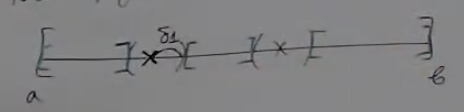
\includegraphics[scale=0.6]{graphic_scheme.png}\caption{Схематичный график функции с $k$ точек разрыва.}\label{Схематичный график функции с $k$ точек разрыва.}
        \end{center}
    \end{figure}
    Дополнение к этому набору интервалов (к набору интервалов окрестностей $k$ точек) - это набор отрезков(отрезки, где нет точек разрыва), на каждом из которых $f(x)$ - непрерывна, а следовательно равномерно непрерывна. А так как число отрезков конечно($k + 1$ штука), то существует $\delta_2$ такое, что если $x', x''$ из какого-то отрезка и $|x' - x''| < \delta_2$, то
    $$
        |f(x') - f(x'')| < \cfrac{\eps}{2(b - a)}
    $$
    Пусть $\delta = \min(\delta_1, \delta_2)$ и $\tau$ - разбиение отрезка $[a, b]$ мелкости меньше $\delta$.
    $$
        \sum_{i = 1}^{n} \omega_i(f)\Delta x_i = \sum'\omega_i(f)\Delta x_i + \sum''\omega_i(f)\Delta x_i
    $$
    где первая сумма - отрезки, не имеющие общих точек с интервалами, а вторая - по всем остальным отрезкам. Поэтому
    $$
        \sum'\omega_i(f)\Delta x_i \leq \cfrac{\eps}{2(b-a)}(b-a) = \cfrac{\eps}{2}
    $$
    Сумма длин оставшихся частей меньше, чем 
    $$
        (\delta + 2\delta_1 + \delta)k \leq \cfrac{\eps}{4C}
    $$
    а значит 
    $$
        \sum''\omega_i(f)\Delta x_i \leq \cfrac{\eps}{4C}2C = \cfrac{\eps}{2}
    $$
    и тогда 
    $$
        \sum_{i = 1}^{n} \omega_i(f)\Delta x_i \leq \eps
    $$
    в итоге получаем требуемое.
\end{proof}
\subsection{Интегрируемость монотонной функции}
\theorem{(об интегрируемости монотонной функции)}{Заданная и монотонная на отрезке $[a, b]$ функция $f(x)$ интегрируема на этом отрезке.}
\begin{proof}
    Рассмотрим два случая:
    \begin{enumerate}
        \item Пусть $f(x) \equiv C$ -  интегрируемость очевидна.
        \item Пусть $f(x) \not \equiv C$ и для определенности не убывает. Пусть $\eps > 0$. Тогда положив $\delta = \cfrac{\eps}{f(b) - f(a)}$ и взяв разбиение $\tau$ отрезка $[a, b]$ мелкости меньше $\delta$, выполняется 
        $$
            \sum_{i = 1}^{n} \omega_i \Delta x_i < \cfrac{\eps}{f(b) - f(a)}\sum_{i = 1}^{n}\omega_i(f) = \cfrac{\eps}{f(b) - f(a)}\sum_{i = 1}^{n}(f(x_i) - f(x_{i-1})) = \eps
        $$
        (кратко: оценили сверху так, что длина всех отрезков меньше eps/(b-a)) \newline 
        Значит, согласно критерию Римана, теорема доказана.
    \end{enumerate}
\end{proof}
\section{Свойства интеграла Римана: линейность; аддитивность по промежутку, монотонность, отделимость от нуля, неравенство с модулем.}
\subsection{Линейность определенного интеграла}
\theorem{(о линейности определенного интеграла)}{Пусть $f, g \in R[a, b]$, тогда}
$$
    \int_{a}^{b} (\alpha f(x) + \beta g(x))dx = \alpha \int_{a}^{b}f(x)dx + \beta \int_{a}^{b} g(x)dx
$$
\begin{proof}
    То, что $\alpha f + \beta g \in R[a, b]$ известно из прошлых теорем. Пусть $I_f = \int_{a}^{b} f(x)dx, I_g = \int_{a}^{b} g(x)dx$. Тогда для разбиения $(\tau, \xi)$ имеем
    $$
        \Bigl| \sigma_\tau(\alpha f + \beta g, \xi) - \alpha I_f - \beta I_g \Bigr| \leq |\alpha| \Bigl| \sigma_\tau(f, \xi) - I_f \Bigr| + |\beta| \Bigl| \sigma_\tau(g, \xi) - I_g \Bigr|
    $$  
    так как $I_f$ и $I_g$ интегрируемы $\Bigl($то есть модули этих разностей, допустим, меньше $\cfrac{\eps}{2|\alpha|}$ и $\cfrac{\eps}{2|\beta|}$$\Bigr)$ получим требуемое.
\end{proof}
\subsection{Аддитивность по промежутку интегрирования}
\theorem{(о аддитивности промежутка интегрирования)}{Пусть $f \in R[a, b], c \in [a, b]$, тогда}
$$
    \int_{a}^{b} f(x)dx = \int_{a}^{c} f(x)dx \int_{c}^{b} f(x)dx
$$
\begin{proof}
    Интегрируемость функциии $f$ на промежутках $[a, c]$ и $[c, b]$ известна. Пусть $\tau$ - разбиение отрезка $[a, b]$, содержащее точку $c$. Тогда оно порождает два разбиения $\tau_1, \tau_2$, причем $\lambda(\tau_1) \leq \lambda(\tau)$ и $\lambda(\tau_2) \leq \lambda(\tau)$. И так как
    $$
        \sum_{[a, b]}^{} f(\xi_i)\Delta x_i = \sum_{[a, c]}^{}f(\xi_i)\Delta x_i + \sum_{[c, b]}^{}f(\xi_i)\Delta x_i
    $$
    и при $\lambda(\tau) \to 0$ получаем требуемое.
\end{proof}
\subsection{Монотонность интеграла}
\theorem{(о монотонности интеграла)}{Пусть $a \leq b, f, g \in R\in[a, b]$, причем $f(x) \leq g(x), x \in [a, b]$, тогда}
$$
    \int_{a}^{b} f(x)dx \leq \int_{a}^{b} g(x)dx
$$
\begin{proof}
    Для интегральных сумм справедливо равенство: 
    $$
        \sum_{i = 1}^{n} f(\xi_i)\Delta x_i \leq \sum_{i = 1}^{n} g(\xi_i)\Delta x_i
    $$
    переходя к пределу при $\lambda(\tau) \to 0$ получаем требуемое.
\end{proof}
.\newline
\textbf{Важное  следствие}
\newline 
Пусть $a \leq b, f \in R[a, b], m = \displaystyle \inf_{x \in [a, b]} f(x), M = sup_{x\in[a,b]}f(x)$, тогда 
$$  
    m(b - a) \leq \int_{a}^{b} f(x)dx \leq M(b - a)
$$  
\subsection{Отделимость от нуля}
\theorem{(об отделимости от нуля)}{Пусть $a < b, f \in R[a, b], f \geq 0$ и существует точка $x_0 \in [a, b]$ такая, что $f(x_0) > 0$, причем $f$ непрерывна в $x_0$. Тогда}
$$
    \int_{a}^{b} f(x)dx > 0
$$
\begin{proof}
    Так как $f(x) > 0$ и $f$ непрерывнав точке $x_0$, то существует окрестность $U(x_0)$, что при $x \in U(x_0)$ выполняется $f(x) > f(x_0)/2$. Тогда в силу монотонности
    $$
        \displaystyle \int_{a}^{b} f(x)dx \geq \int_{[a, b] \cap U(x_0)}^{} f(x)dx > \cfrac{f(x_0)}{2} + \int_{[a, b] \cap U(x_0)}^{} f(x)dx > 0
    $$
\end{proof}
\subsection{Неравенство с модулем}
\theorem{(о неравенстве с модулем)}{Пусть $f \in R[a, b]$, тогда}
$$
    \Biggl| \int_{a}^{b} f(x)dx \Biggr| \leq \Biggl| \int_{a}^{b}|f(x)|dx \Biggr| 
$$
\begin{proof}
    Интегрируемость функции $|f|$ известна. А так как 
    $$
        \Biggl| \sum_{i = 1}^{n} f(\xi_i)\Delta x_i \Biggr| \leq \Biggl| \sum_{i = 1}^{n}|f(\xi_i)|\Delta x_i \Biggr|
    $$
    то переходя к пределам получим требуемое.
\end{proof}
\section{Первая теорема о среднем}
\theorem{(первая теорема о среднем)}{Пусть $f, g \in R[a, b], g(x)$ не меняет знак на $[a, b], m = \inf f(x), M = \sup f(x)$, тогда}
$$
    \exists \mu \in [m, M]: \; \int_{a}^{b} f(x)g(x)dx = \mu\int_{a}^{b} g(x)dx
$$
Кроме того, если $f(x) \in C[a, b]$, то
$$
    \exists \xi \in [a, b]: \; \int_{a}^{b}f(x)g(x)dx = f(\xi)\int_{a}^{b}g(x)dx
$$
\begin{proof}
    Пусть $g(x) \geq 0$ на отрезке $[a, b]$, тогда
    $$
        mg(x) \leq f(x)g(x) \leq Mg(x), \; x \in [a, b]
    $$
    и по монотонности интеграла
    $$
        m\int_{a}^{b}g(x)dx \leq \int_{a}^{b}f(x)g(x)dx \leq M\int_{a}^{b}g(x)dx
    $$
    Если $\int_{a}^{b} g(x)dx = 0$, то $\mu$ - любое число отрезка. А если $\int_{a}^{b}g(x)dx \neq 0$, то $\int_{a}^{b} g(x)dx > 0$ и, поделив на этот интеграл получим
    $$
        m \leq \cfrac{\int_{a}^{b}f(x)g(x)dx}{\int_{a}^{b}g(x)dx} \leq M
    $$
    Тогда пусть $\mu = \cfrac{\int_{a}^{b}f(x)g(x)dx}{\int_{a}^{b}g(x)dx}$ (напомним, интеграл - это какое-то число). 
    \newline \newline 
    Если $f \in C[a, b]$, то по теореме Больцано-Коши для каждого $\mu \in [m, M]$ существует $\xi \in [a, b]$, что $f(\xi) = \mu$.
\end{proof}
\section{Интеграл с переменным верхним пределом: определение, непрерывность, дифференциируемость (две теоремы).}
\definition{Пусть $f \in R[a, b]$ и $x \in [a, b]$. Функция}
$$
    \Phi(x) = \int_{a}^{x} f(x)dx
$$
называется \textbf{интегралом с переменным верхним пределом}.
\subsection{Непрерывность $\Phi(x)$}
\theorem{(о непрерывности $\Phi(x)$)}{}
$$
    \Phi(x) \in C[a, b]
$$
\begin{proof}
    Пусть $x_0 \in [a, b], x_0 + \Delta x \in [a, b]$. Так как функция $f \in R[a, b]$, то она ограничена на отрезке, то есть 
    $$
        |f(x)| \leq C, \; x \in [a, b]
    $$
    и тогда 
    $$
        |\Phi(x_0 + \Delta x) - \Phi(x_0)| = \Biggl| \int_{x_0}^{x_0 + \Delta x} f(x)dx \Biggr| \leq \Biggl| \int_{x_0}^{x_0 + \Delta x} |f(x)|dx \Biggr| \leq 
    $$
    $$
        \leq \Biggl| \int_{x_0}^{x_0 + \Delta x} Cdx \Biggr| = C |\Delta x|
    $$
    значит при $\Delta x \to 0$ выполняется $\Phi(x_0 + \Delta x) \to \Phi(x_0)$, что и означает непрерывность функции в точке $x_0$, а так как $x_0$ - произвольная точка $[a, b]$, то утверждение доказано.
\end{proof}
\subsection{Дифференцируемость $\Phi(x)$}
\theorem{(о дифференцируемости $\Phi(x)$ или т.Барроу)}{$\Phi(x)$ дифференцируема в точках непрерывности функции $f(x)$, причем}
$$
    (\Phi(x))'(x_0) = f(x_0)
$$
\begin{proof}
    Пусть $f(x)$ непрерывна в точке $x_0$ и $x_0 + \Delta x \in [a, b]$.
    $$
        \Biggl| \cfrac{\Phi(x_0 + \Delta x) - \Phi(x)}{\Delta x} - f(x_0) \Biggr| = \Biggl| \cf{\int_{x_0}^{x_0 + \D x} f(x)dx - f(x_0)\D x}{\D x} \Biggr| =
    $$
    $$
        \Biggl| \cf{\int_{x_0}^{x_0 + \D x} (f(x) - f(x_0))dx}{\D x} \Biggr|
    $$
    (последний переход - сворачивание $f(x_0)\D x$ как интеграла по такому же промежутку)
    \newline 
    Пусть $\eps > 0$, тогда (так как $f(x)$ непрерывна)
    $$
        \exists \delta > 0: \; \forall x \in [a, b]: \; |x - x_0| < \delta \Rightarrow |f(x) - f(x_0)| < \eps
    $$
    Пусть $\D x < \delta$ ($x - x_0 < \delta$), тогда 
    $$
        \Biggl| \cf{\int_{x_0}^{x_0 + \D x} (f(x) - f(x_0))dx}{\D x} \Biggr| \leq \Biggl| \cf{\int_{x_0}^{x_0 + \D x} |f(x) - f(x_0)|dx}{\D x} \Biggr| < \Biggl| \cf{\int_{x_0}^{x_0 + \D x} \eps \cdot dx}{\D x} \Biggr| = \eps
    $$
    что означает, что (по определению производной)
    $$
        \displaystyle \limToZero{\D x}{\cf{\Phi(x_0 + \D x) - \Phi(x_0)}{\D x}} = f(x_0)
    $$
\end{proof}
\section{Формула Ньютона-Лейбница. Усиленная формула и обобщенная формула.}
\subsection{Формула Ньютона-Лейбница}
\theorem{(Формула Ньютона-Лейбница)}{Пусть $f(x) \in C[a, b]$ и $F(x)$ - ее первообразная. Тогда}
$$
    \int_{a}^{b} f(x)dx = F(x)\Bigr|_{a}^{b} = F(b) - F(a)
$$  
\begin{proof}
    Любая первообразная непрерывной функции имеет вид: 
    $$
        F(x) = \int_{a}^{x} f(x)dx + C
    $$
    Так как 
    $$
        F(A) = \int_{a}^{a} f(x)dx + C = C
    $$
    то $C = F(a)$. Положив в равенстве
    $$
        F(x) = \int_{a}^{x} f(x)dx + F(a)
    $$
    то при $x = b$ получается 
    $$
        F(b) = \int_{a}^{b} f(x)dx + F(a) \Rightarrow \int_{a}^{b} f(x)dx = F(b) - F(a)
    $$
\end{proof}
\subsection{Усиленная формула Ньютона-Лейбница}
\theorem{(Усиленная формула Ньютона-Лейбница)}{Пусть $f \in R[a, b]$ и существует некоторая первообразная $F(x)$ на $[a, b]$, тогда}
$$
    \int_{a}^{b} f(x)dx = F(x)\Bigr|_{a}^{b} = F(b) - F(a)
$$
\begin{proof}
    Пусть $x_k = a + \cf{k(b - a)}{n}$, $k \in \{ 0, 1, 2, \dots, n \}$ - разбиение (кстати равномерное) отрезка. Тогда 
    $$
        F(b) - F(a) = F(x_n) - F(x_0) = \sum_{k = 1}^{n} (F(x_k) - F(x_{k - 1}))
    $$
    Согласно теореме Лагранжа, существует $\xi^n_k \in (x_k, x_{k - 1})$ такое, что
    $$
        F(x_k) - F(x_{k - 1}) = f(\xi_k^n)(x_k - x_{k - 1})
    $$
    а тогда 
    $$
        F(b) - F(a) = \sum_{k = 1}^{n} f(\xi_k^n)\D x_k
    $$
    перейдя к пределу с $n \to +\infty$ получим
    $$
        \limToInf{n}{\sum_{k = 1}^{n}f(\xi_k^n)\D x_k} = \int_{a}^{b}f(x)dx
    $$
    что и завершает доказательство.
\end{proof}
Эта формула работает для любой первообразной $f(x)$.
\subsection{Обобщенная формула Ньютона-Лейбница}
\theorem{(Обобщение формулы Ньютона-Лейбница)}{Пусть $f(x) \in R[a, b]$ и $F(x)$ - обобщенная первообразная функции $f(x)$, тогда}
$$
    \int_{a}^{b}f(x)dx = F(b) - F(a)
$$ 
\begin{proof}
    Пусть $\alpha_1, \alpha_2, \dots, \alpha_{k-1}$ - точки внутри $(a, b)$, в которых нарушено $F'(x) = f(x)$. Добавим к ним $\alpha_0 = a$, $\alpha_k = b$. Так как интеграл - непрерывная функция по обоим пределам, то
    $$
        \int_{\alpha_{p - 1}}^{\alpha_p} f(x)dx = \limToZero{\eps}{\int_{\alpha_{p-1} + \eps}^{\alpha_p - \eps} f(x)dx} = \limToZero{\eps}{(F(\alpha_p - \eps) - F(\alpha_{p - 1} + \eps))} = 
    $$
    $$
        = F(\alpha_p) - F(\alpha_{p - 1})
    $$
    где последнее - так как функция непрерывна. Тогда 
    $$
        \int_{a}^{b} f(x)dx = \sum_{p = 1}^{k} \int_{\alpha_{p-1}}^{\alpha_p}f(x)dx = \sum_{p = 1}^{k} F(\alpha_p) - F(\alpha_{p - 1}) = 
    $$
    $$
        F(\alpha_k) - F(\alpha_0) = F(b) - F(a)
    $$
\end{proof}
\section{Формула интегрирования по частям. Формула замены переменной.}
\subsection{Формула интегрирования по частям}
\theorem{(формула интегрирования по частям)}{Пусть $u, v$ - дифференцируемы на $[a, b]$, причем $u', v' \in R[a, b]$, тогда}
$$
    \int_{a}^{b} udv = uv\Bigr|^{b}_{a} - \int_{a}^{b} vdu
$$
\begin{proof}
    Очевидно, что $uv' \in R[a, b]$ и $u'v \in R[a, b]$. Кроме того, $(uv)' = u'v + v'u \in R[a, b]$, а значит, по усиленной формуле Ньютона-Лейбница
    $$
        \int_{a}^{b}u'vdx + \int_{a}^{b}uv'dx = \int_{a}^{b}(u'v + v'u)dx = \int_{a}^{b}(uv)'dx = uv\Bigr|^{a}_{b}
    $$
\end{proof}
\subsection{Формула замены переменной}
\theorem{(формула замены переменной)}{Пусть $f(x) \in C[a, b], x = \phi(t)\;:\; [\alpha, \beta] \to [a, b], \phi(t)$ дифференцируема и $\phi'(t) \in R[\alpha, \beta]$, тогда}
$$
    \int_{\phi(\alpha)}^{\phi(\beta)} f(x)dx = \int_{\alpha}^{\beta} f(\phi(t))\phi'(t)dt
$$
\begin{proof}
    Интеграл от правой части определен. По свойствам интегрируемых функций $f(\phi(t))\phi'(t) \in R[\alpha, \beta]$, причем $F(\phi(t))$ - первообразная этой функции, если $F(x)$ - первообразная $f(x)$. Тогда
    $$
        \int_{\alpha}^{\beta} f(\phi(t))\phi'(t)dt = F(\phi(\beta)) - F(\phi(\alpha)) = \int_{\phi(\alpha)}^{\phi(\beta)} f(x)dx
    $$
\end{proof}
\section{Интеграл от четной, нечетной и периодический функции. Изменение функции в конечном числе точек.}
\subsection{Интеграл четной функции}
\theorem{}{Пусть $f \in R[0, a]$ и является четной. Тогда}
$$
    \int_{-a}^{a} f(x)dx = 2\int_{0}^{a} f(x)dx
$$
\begin{proof}
    Функция четна $(f(-x) = f(x))$, значит $f \in R[-a, a]$.
    $$
        \int_{-a}^{a}f(x)dx = \int_{-a}^{0}f(x)dx + \int_{0}^{a}f(x)dx 
    $$
    В первом интеграле замена $t = -x, \; dt = -dx$
    $$
        \int_{-a}^{a} f(x)dx = \int_{0}^{a} f(t)dt + \int_{0}^{a}f(x)dx = 2\int_{0}^{a} f(x)dx 
    $$
\end{proof}
\subsection{Интеграл нечетной функции}
\theorem{}{Пусть $f \in R[0, a]$ и является нечетной. Тогда}
$$
    \int_{-a}^{a}f(x)dx = 0
$$  
\begin{proof}
    аналогично четной функции, но при замене $f(t) = -f(t)$ и минус не уйдет.
\end{proof}
\subsection{Интеграл периодической функции}
\theorem{}{Пусть $f \in R[0, T]$ и является периодической с периодом $T$. Тогда}
$$
    \int_{a}^{a + T} f(x)dx = \int_{0}^{T}f(x)dx, \; a \in \R
$$
\begin{proof}
    Сделаем замену $t = x - a$
    $$
        \int_{a}^{a + T} f(x)dx = \int_{0}^{T} f(t)dt
    $$
\end{proof}
\subsection{Теорема об изменении функции в конечном числе точек}
\theorem{(об изменении функции в конечном числе точек)}{Пусть $g \in R[a, b], f: [a, b] \to \R, f(x) = g(x)$ для $\forall x \in [a, b]$ кроме конечного числа точек. Тогда }
$$
    \int_{a}^{b}g(x)dx = \int_{a}^{b}f(x)dx
$$
\begin{proof}
    Пусть $f(x) = g(x)$ на $[a, b]$ везде, кроме точки $c$. Построим интегральную сумму для $f$
    $$
        \sigma_\tau (f, \xi) = \sum_{i = j}^{} f(\xi_i)\D x_i + f(\xi_j)\D x_j
    $$
    тогда, так как $f = g$ везде, кроме $c$
    $$
        \sigma_\tau(f, \xi) = \sigma_\tau(g, \xi) - g(\xi_j)\D x_j + f(\xi_j)\D x_j
    $$
    перейдя к пределу при $\lambda(\tau) \to 0$
    $$
        I = I - 0 + 0 = I
    $$
\end{proof}
%\section{Площадь фигуры. Свойства площади. Площадь криволинейной трапеции и фигуры, ограниченной графиками двух функций и вертикальными линиями.}
\end{document}